% Options for packages loaded elsewhere
\PassOptionsToPackage{unicode}{hyperref}
\PassOptionsToPackage{hyphens}{url}
\PassOptionsToPackage{dvipsnames,svgnames,x11names}{xcolor}
%
\documentclass[
  letterpaper,
  DIV=11,
  numbers=noendperiod]{scrartcl}

\usepackage{amsmath,amssymb}
\usepackage{iftex}
\ifPDFTeX
  \usepackage[T1]{fontenc}
  \usepackage[utf8]{inputenc}
  \usepackage{textcomp} % provide euro and other symbols
\else % if luatex or xetex
  \usepackage{unicode-math}
  \defaultfontfeatures{Scale=MatchLowercase}
  \defaultfontfeatures[\rmfamily]{Ligatures=TeX,Scale=1}
\fi
\usepackage{lmodern}
\ifPDFTeX\else  
    % xetex/luatex font selection
\fi
% Use upquote if available, for straight quotes in verbatim environments
\IfFileExists{upquote.sty}{\usepackage{upquote}}{}
\IfFileExists{microtype.sty}{% use microtype if available
  \usepackage[]{microtype}
  \UseMicrotypeSet[protrusion]{basicmath} % disable protrusion for tt fonts
}{}
\makeatletter
\@ifundefined{KOMAClassName}{% if non-KOMA class
  \IfFileExists{parskip.sty}{%
    \usepackage{parskip}
  }{% else
    \setlength{\parindent}{0pt}
    \setlength{\parskip}{6pt plus 2pt minus 1pt}}
}{% if KOMA class
  \KOMAoptions{parskip=half}}
\makeatother
\usepackage{xcolor}
\setlength{\emergencystretch}{3em} % prevent overfull lines
\setcounter{secnumdepth}{-\maxdimen} % remove section numbering
% Make \paragraph and \subparagraph free-standing
\makeatletter
\ifx\paragraph\undefined\else
  \let\oldparagraph\paragraph
  \renewcommand{\paragraph}{
    \@ifstar
      \xxxParagraphStar
      \xxxParagraphNoStar
  }
  \newcommand{\xxxParagraphStar}[1]{\oldparagraph*{#1}\mbox{}}
  \newcommand{\xxxParagraphNoStar}[1]{\oldparagraph{#1}\mbox{}}
\fi
\ifx\subparagraph\undefined\else
  \let\oldsubparagraph\subparagraph
  \renewcommand{\subparagraph}{
    \@ifstar
      \xxxSubParagraphStar
      \xxxSubParagraphNoStar
  }
  \newcommand{\xxxSubParagraphStar}[1]{\oldsubparagraph*{#1}\mbox{}}
  \newcommand{\xxxSubParagraphNoStar}[1]{\oldsubparagraph{#1}\mbox{}}
\fi
\makeatother


\providecommand{\tightlist}{%
  \setlength{\itemsep}{0pt}\setlength{\parskip}{0pt}}\usepackage{longtable,booktabs,array}
\usepackage{calc} % for calculating minipage widths
% Correct order of tables after \paragraph or \subparagraph
\usepackage{etoolbox}
\makeatletter
\patchcmd\longtable{\par}{\if@noskipsec\mbox{}\fi\par}{}{}
\makeatother
% Allow footnotes in longtable head/foot
\IfFileExists{footnotehyper.sty}{\usepackage{footnotehyper}}{\usepackage{footnote}}
\makesavenoteenv{longtable}
\usepackage{graphicx}
\makeatletter
\newsavebox\pandoc@box
\newcommand*\pandocbounded[1]{% scales image to fit in text height/width
  \sbox\pandoc@box{#1}%
  \Gscale@div\@tempa{\textheight}{\dimexpr\ht\pandoc@box+\dp\pandoc@box\relax}%
  \Gscale@div\@tempb{\linewidth}{\wd\pandoc@box}%
  \ifdim\@tempb\p@<\@tempa\p@\let\@tempa\@tempb\fi% select the smaller of both
  \ifdim\@tempa\p@<\p@\scalebox{\@tempa}{\usebox\pandoc@box}%
  \else\usebox{\pandoc@box}%
  \fi%
}
% Set default figure placement to htbp
\def\fps@figure{htbp}
\makeatother

\usepackage{booktabs}
\usepackage{longtable}
\usepackage{array}
\usepackage{multirow}
\usepackage{wrapfig}
\usepackage{float}
\usepackage{colortbl}
\usepackage{pdflscape}
\usepackage{tabu}
\usepackage{threeparttable}
\usepackage{threeparttablex}
\usepackage[normalem]{ulem}
\usepackage{makecell}
\usepackage{xcolor}
\usepackage{tabularray}
\usepackage[normalem]{ulem}
\usepackage{graphicx}
\UseTblrLibrary{booktabs}
\UseTblrLibrary{rotating}
\UseTblrLibrary{siunitx}
\NewTableCommand{\tinytableDefineColor}[3]{\definecolor{#1}{#2}{#3}}
\newcommand{\tinytableTabularrayUnderline}[1]{\underline{#1}}
\newcommand{\tinytableTabularrayStrikeout}[1]{\sout{#1}}
\KOMAoption{captions}{tableheading}
\usepackage{float}
\floatplacement{table}{H}
\makeatletter
\@ifpackageloaded{caption}{}{\usepackage{caption}}
\AtBeginDocument{%
\ifdefined\contentsname
  \renewcommand*\contentsname{Table of contents}
\else
  \newcommand\contentsname{Table of contents}
\fi
\ifdefined\listfigurename
  \renewcommand*\listfigurename{List of Figures}
\else
  \newcommand\listfigurename{List of Figures}
\fi
\ifdefined\listtablename
  \renewcommand*\listtablename{List of Tables}
\else
  \newcommand\listtablename{List of Tables}
\fi
\ifdefined\figurename
  \renewcommand*\figurename{Figure}
\else
  \newcommand\figurename{Figure}
\fi
\ifdefined\tablename
  \renewcommand*\tablename{Table}
\else
  \newcommand\tablename{Table}
\fi
}
\@ifpackageloaded{float}{}{\usepackage{float}}
\floatstyle{ruled}
\@ifundefined{c@chapter}{\newfloat{codelisting}{h}{lop}}{\newfloat{codelisting}{h}{lop}[chapter]}
\floatname{codelisting}{Listing}
\newcommand*\listoflistings{\listof{codelisting}{List of Listings}}
\makeatother
\makeatletter
\makeatother
\makeatletter
\@ifpackageloaded{caption}{}{\usepackage{caption}}
\@ifpackageloaded{subcaption}{}{\usepackage{subcaption}}
\makeatother

\usepackage{bookmark}

\IfFileExists{xurl.sty}{\usepackage{xurl}}{} % add URL line breaks if available
\urlstyle{same} % disable monospaced font for URLs
\hypersetup{
  pdftitle={Homework 5},
  pdfauthor={Answer Key},
  colorlinks=true,
  linkcolor={blue},
  filecolor={Maroon},
  citecolor={Blue},
  urlcolor={Blue},
  pdfcreator={LaTeX via pandoc}}


\title{Homework 5}
\usepackage{etoolbox}
\makeatletter
\providecommand{\subtitle}[1]{% add subtitle to \maketitle
  \apptocmd{\@title}{\par {\large #1 \par}}{}{}
}
\makeatother
\subtitle{Research Methods, Spring 2025}
\author{Answer Key}
\date{}

\begin{document}
\maketitle


\begin{enumerate}
\def\labelenumi{\arabic{enumi}.}
\tightlist
\item
  Plot the share of the adult population with direct purchase health
  insurance over time.
\end{enumerate}

\pandocbounded{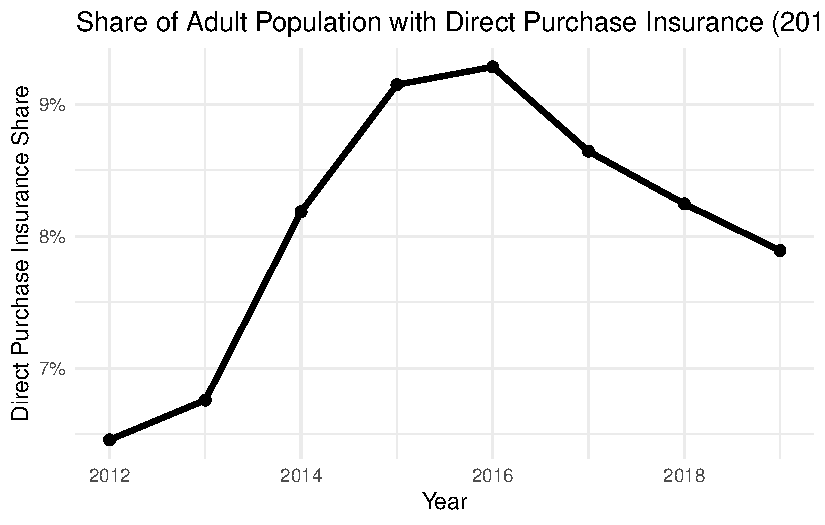
\includegraphics[keepaspectratio]{debell-g-5-2_files/figure-pdf/unnamed-chunk-3-1.pdf}}

\begin{enumerate}
\def\labelenumi{\arabic{enumi}.}
\setcounter{enumi}{1}
\tightlist
\item
  Discuss the reduction in direct purchase health insurance in later
  years. Can you list a couple of policies that might have affected the
  success of the direct purchase insurance market?
\end{enumerate}

Since 2016, the share of adults with direct purchase insurance has
decreased. The Tax Cuts and Jobs Act of 2017 eliminated the penalty for
not having insurance starting in 2019. Without this mandate, fewer
healthy individuals opted into coverage because there was no penalty.

\begin{enumerate}
\def\labelenumi{\arabic{enumi}.}
\setcounter{enumi}{2}
\tightlist
\item
  Plot the share of the adult population with Medicaid over time.
\end{enumerate}

\pandocbounded{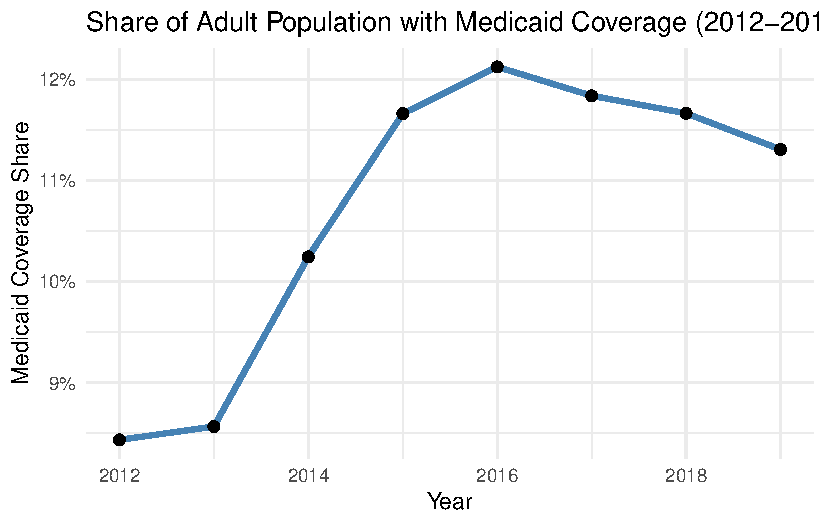
\includegraphics[keepaspectratio]{debell-g-5-2_files/figure-pdf/unnamed-chunk-4-1.pdf}}

\begin{enumerate}
\def\labelenumi{\arabic{enumi}.}
\setcounter{enumi}{3}
\tightlist
\item
  Plot the share of uninsured over time, separately by states that
  expanded Medicaid in 2014 versus those that did not. Drop all states
  that expanded after 2014.
\end{enumerate}

\pandocbounded{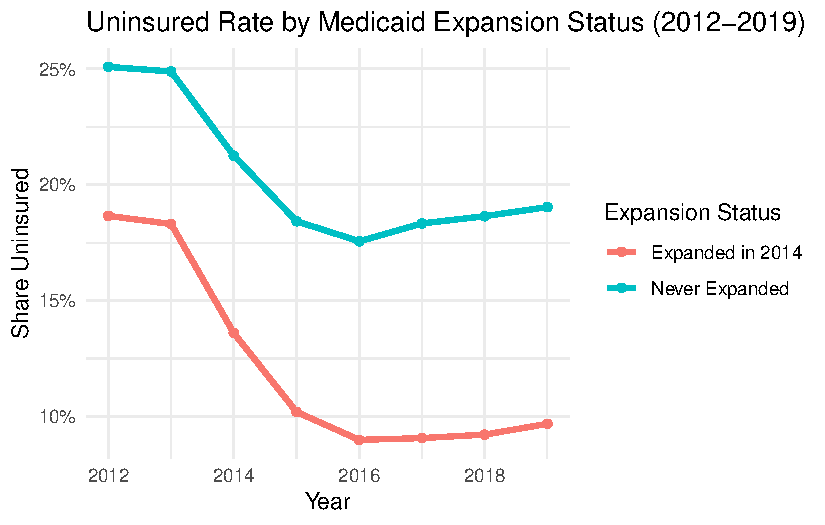
\includegraphics[keepaspectratio]{debell-g-5-2_files/figure-pdf/unnamed-chunk-5-1.pdf}}

\begin{enumerate}
\def\labelenumi{\arabic{enumi}.}
\setcounter{enumi}{4}
\tightlist
\item
  Calculate the average percent of uninsured individuals in 2012 and
  2015, separately for expansion and non-expansion states. Present your
  results in a basic 2x2 DD table.
\end{enumerate}

\begin{table}

\caption{Table 1: Difference-in-Differences Table of Average Uninsured Rate}
\centering
\begin{tabular}[t]{lrr}
\toprule
Group & Pre & Post\\
\midrule
Expanded in 2014 & 0.19 & 0.10\\
Never Expanded & 0.25 & 0.18\\
\bottomrule
\end{tabular}
\end{table}

\begin{enumerate}
\def\labelenumi{\arabic{enumi}.}
\setcounter{enumi}{5}
\tightlist
\item
  Estimate the effect of Medicaid expansion on the uninsurance rate
  using a standard DD regression estimator, again focusing only on
  states that expanded in 2014 versus those that never expanded.
\end{enumerate}

\begin{table}
\centering
\begin{talltblr}[         %% tabularray outer open
caption={Table 2: DD Estimates for Medicaid Expansion},
note{}={+ p \num{< 0.1}, * p \num{< 0.05}, ** p \num{< 0.01}, *** p \num{< 0.001}},
]                     %% tabularray outer close
{                     %% tabularray inner open
colspec={Q[]Q[]},
column{2}={}{halign=c,},
column{1}={}{halign=l,},
hline{10}={1,2}{solid, black, 0.05em},
}                     %% tabularray inner close
\toprule
& (1) \\ \midrule %% TinyTableHeader
(Intercept) & \num{0.211}*** \\
& (\num{0.009}) \\
treat & \num{-0.044}*** \\
& (\num{0.011}) \\
post & \num{-0.052}*** \\
& (\num{0.011}) \\
treat × post & \num{-0.021}+ \\
& (\num{0.013}) \\
Num.Obs. & \num{304} \\
R2 & \num{0.455} \\
R2 Adj. & \num{0.449} \\
AIC & \num{-1034.5} \\
BIC & \num{-1019.6} \\
RMSE & \num{0.04} \\
Std.Errors & IID \\
\bottomrule
\end{talltblr}
\end{table}

\begin{enumerate}
\def\labelenumi{\arabic{enumi}.}
\setcounter{enumi}{6}
\tightlist
\item
  Include state and year fixed effects in your estimates. Try using the
  lfe or fixest package to estimate this instead of directly including
  the fixed effects.
\end{enumerate}

\begin{verbatim}
The variables 'treat' and 'post' have been removed because of collinearity (see $collin.var).
\end{verbatim}

\begin{verbatim}
OLS estimation, Dep. Var.: uninsured_rate
Observations: 304
Fixed-effects: State: 38,  year: 8
Standard-errors: Clustered (State) 
            Estimate Std. Error  t value Pr(>|t|)    
treat:post -0.021149   0.008934 -2.36732 0.023259 *  
... 2 variables were removed because of collinearity (treat and post)
---
Signif. codes:  0 '***' 0.001 '**' 0.01 '*' 0.05 '.' 0.1 ' ' 1
RMSE: 0.013938     Adj. R2: 0.934467
                 Within R2: 0.08155 
\end{verbatim}

\begin{enumerate}
\def\labelenumi{\arabic{enumi}.}
\setcounter{enumi}{7}
\tightlist
\item
  Repeat the analysis in question 7 but include all states (even those
  that expanded after 2014). Are your results different? If so, why?
\end{enumerate}

\begin{verbatim}
OLS estimation, Dep. Var.: perc_unins
Observations: 416
Fixed-effects: State: 52,  year: 8
Standard-errors: Clustered (State) 
       Estimate Std. Error t value   Pr(>|t|)    
treat -0.023766   0.005602 -4.2423 9.3304e-05 ***
---
Signif. codes:  0 '***' 0.001 '**' 0.01 '*' 0.05 '.' 0.1 ' ' 1
RMSE: 0.013106     Adj. R2: 0.937003
                 Within R2: 0.155529
\end{verbatim}

\begin{enumerate}
\def\labelenumi{\arabic{enumi}.}
\setcounter{enumi}{8}
\tightlist
\item
  Provide an ``event study'' graph showing the effects of Medicaid
  expansion in each year. Use the specification that includes state and
  year fixed effects, limited to states that expanded in 2014 or never
  expanded.
\end{enumerate}

\pandocbounded{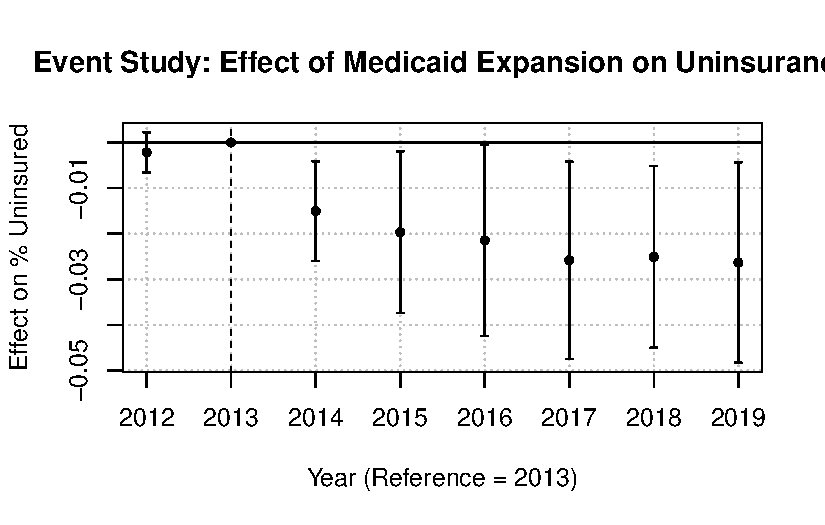
\includegraphics[keepaspectratio]{debell-g-5-2_files/figure-pdf/unnamed-chunk-10-1.pdf}}

\begin{enumerate}
\def\labelenumi{\arabic{enumi}.}
\setcounter{enumi}{9}
\tightlist
\item
  Repeat part 9 but again include states that expanded after 2014. Note:
  this is tricky\ldots you need to put all states onto ``event time'' to
  create this graph.
\end{enumerate}

\pandocbounded{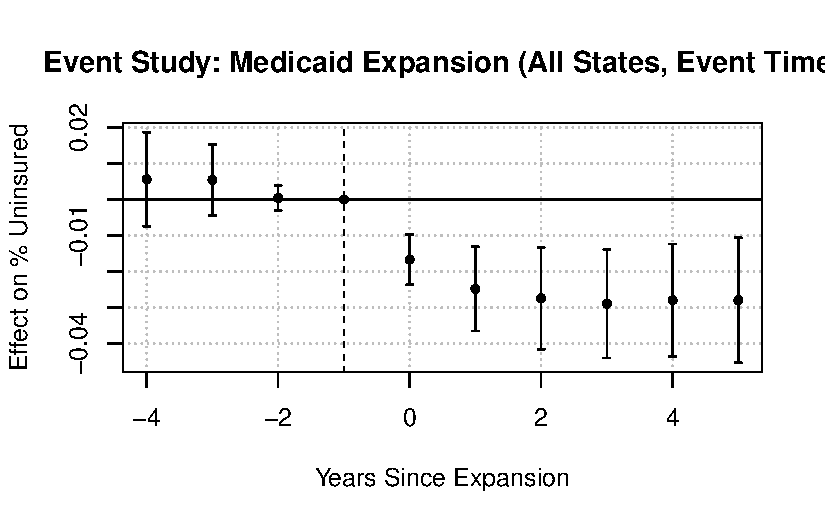
\includegraphics[keepaspectratio]{debell-g-5-2_files/figure-pdf/unnamed-chunk-11-1.pdf}}




\end{document}
